\documentclass{article}%
\usepackage[T1]{fontenc}%
\usepackage[utf8]{inputenc}%
\usepackage{lmodern}%
\usepackage{textcomp}%
\usepackage{lastpage}%
\usepackage[head=40pt,margin=0.5in,bottom=0.6in]{geometry}%
\usepackage{graphicx}%
%
\title{\textbf{Denuncian que no hay transporte en urbanización Nueva Casarapa de Guarenas}}%
\author{Diario El Universal}%
\date{01/10/2018}%
%
\begin{document}%
\normalsize%
\maketitle%
\textbf{URL: }%
http://www.eluniversal.com/caracas/22031/denuncian{-}que{-}no{-}hay{-}transporte{-}en{-}urbanizacion{-}nueva{-}casarapa{-}de{-}guarenas\newline%
%
\textbf{Periodico: }%
EU, %
ID: %
22031, %
Seccion: %
caracas\newline%
%
\textbf{Palabras Claves: }%
NO\_TIENE\newline%
%
\textbf{Derecho: }%
2.3, %
Otros Derechos: %
, %
Sub Derechos: %
2.3.1\newline%
%
\textbf{EP: }%
SI\newline%
\newline%
%
\textbf{\textit{Usuarios protestaron en Parque Miranda debido a que los transportistas cobran el pasaje en 10 bolívares soberanos. Alertaron que los choferes decidieron no trabajar este lunes.}}%
\newline%
\newline%
%
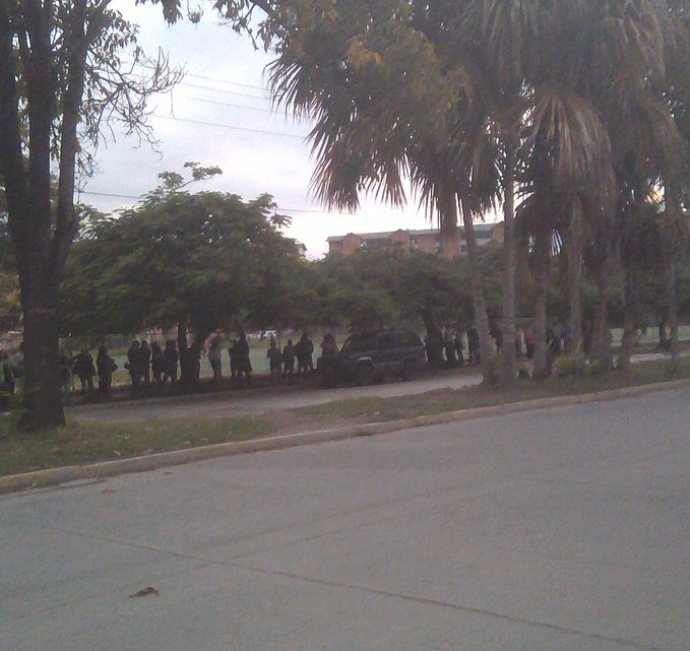
\includegraphics[width=300px]{62.jpg}%
\newline%
%
A las 6 de la mañana ya se formaron largas colas de usuarios para esperar las unidades de transporte público en la urbanización Nueva Casarapa en Guarenas, según denunciaron.%
\newline%
%
JOSÉ ANDRADE GODOY%
\newline%
%
Los usuarios exigieron, a través de la red social Twitter, la intervención de las autoridades correspondientes para solucionar la situación, "porque no hay transporte para Caracas", alertaron.%
\newline%
%
Señalaron que durante el fin de semana, en la parada del Parque Francisco de Miranda los pasajeros protestaron debido a que los transportistas cobran el pasaje en 10 bolívares soberanos para la ruta Guarenas{-} Guatire.%
\newline%
%
\end{document}